\documentclass[11pt,fleqn]{article}

%% This first part is the document header, which you don't need to edit.
%% Scroll down to \begin{document}

\usepackage[latin1]{inputenc}
\usepackage{enumerate}
\usepackage[hang,flushmargin]{footmisc}
\usepackage{amsmath}
\usepackage{amsfonts}
\usepackage{amssymb}
\usepackage{amsthm}
\usepackage{graphicx}
\usepackage{hyperref}
\usepackage{tcolorbox}
\definecolor{mycolor}{rgb}{0.122, 0.435, 0.698}
\newtcbox{\mybox}{nobeforeafter,colframe=mycolor,colback=mycolor!10!white,boxrule=0.5pt,arc=4pt,boxsep=0pt,left=6pt,right=6pt,top=6pt,bottom=6pt,tcbox
raise base}


\theoremstyle{definition}
\newtheorem{theorem}{Theorem}[section]
\newtheorem{lemma}[theorem]{Lemma}
\newtheorem{corollary}[theorem]{Corollary}
\newtheorem{proposition}[theorem]{Proposition}
\newtheorem{definition}[theorem]{Definition}
\newtheorem{example}[theorem]{Example}

\setlength{\oddsidemargin}{0px}
\setlength{\textwidth}{460px}
\setlength{\voffset}{-1.5cm}
\setlength{\textheight}{20cm}
\setlength{\parindent}{0px}
\setlength{\parskip}{10pt}

\begin{document}

\topskip0pt
\vspace*{\fill}
\begin{center}
{\Huge
Guide to \hspace{4.4cm} \texttt{ }
}\\

\includegraphics[scale=0.6]{GitHubLogo.jpg}
\end{center}
\begin{center}
\texttt{ } \newline
\texttt{ } \newline
Ethan Cheng, Yicheng Wang
\end{center}
\vspace*{\fill}

\newpage
\tableofcontents

\newpage
\section{Introduction}
I made this guide because GitHub is an awesome tool, but using it incorrectly
will cause a lot of problems. This guide is to serve as a tutorial and a
reference for people using GitHub.

\section{Installation}
\subsection{Windows}
There are two ways of using GitHub on Windows. One way is via the graphical
interface available for download here: \url{https://desktop.github.com}.
However, most of the sections of this guide will be focused on command-line
versions of \texttt{Git}, so we'll be using the second way of using GitHub on
Windows: \textbf{Git Bash}, available for download here:
\url{https://git-for-windows.github.io} and here:
\url{http://git-scm.com/download/win}. (Yes, for those reading the original PDF
version of this guide, these links are clickable.) Once you have downloaded it,
run the installer. (The following pictures might look a bit different on your
computer since I'm running Windows off Parallels, but most of the content is the
same.)

\begin{enumerate}[Step 1.]
\item When you open the installer, you should see this:
\begin{center}
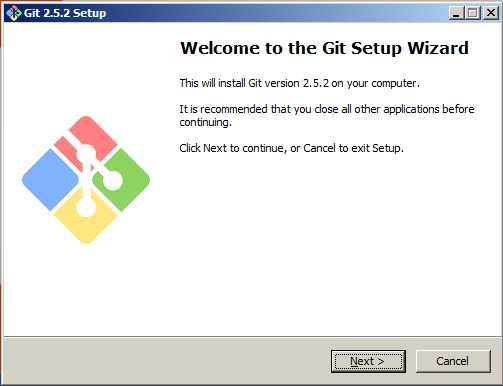
\includegraphics[scale=0.6]{gitwininstall1.png}
\end{center}
Click "Next."

\item The next step is the GNU GPL for GitHub. You could take the time to read
    this... but in any case, just hit ``Next.''
\begin{center}
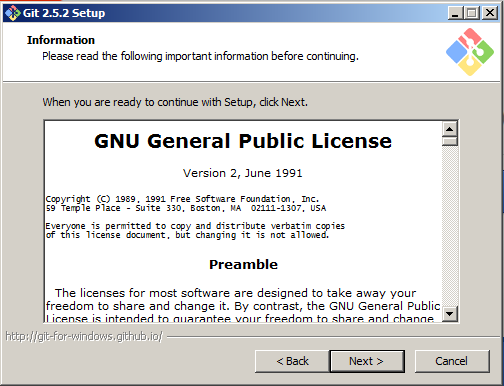
\includegraphics[scale=0.6]{gitwininstall2.png}
\end{center}

\item Different operating systems represent `newline' characters in different
    ways: it's why sometimes when you open code in Windows, everything is on a
    single line. Windows-style line endings are \verb|'\n\r'| and Unix-style
    line endings are \verb|'\n'|. For most cases, you want to select the
    `Checkout Windows-style, commit Unix-style' option.
\begin{center}
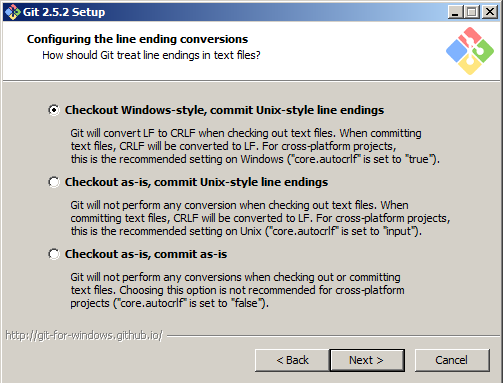
\includegraphics[scale=0.6]{gitwininstall3.png}
\end{center}

\item The Windows Command Prompt is known to be a pretty annoying interface.
    It's not freely resizable, it has very bad scrollback, and doesn't work well
    with a lot of things. Git Bash includes a version of TTY as its interface.
    Select `MinTTY' if you don't want to deal with CMD when working with Git.
\begin{center}
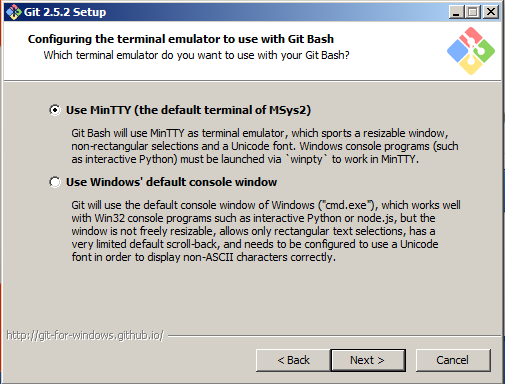
\includegraphics[scale=0.6]{gitwininstall4.png}
\end{center}

\item The next step is experimental features. Use these at your own risk.
\begin{center}
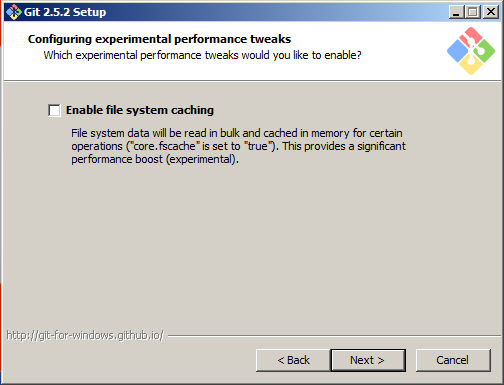
\includegraphics[scale=0.6]{gitwininstall5.png}
\end{center}

\item You can change the Git installation folder, but like with most Windows
    programs, it's best to leave the default value.
\begin{center}
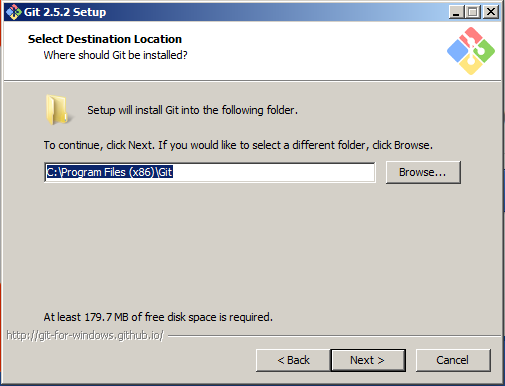
\includegraphics[scale=0.6]{gitwininstall6.png}
\end{center}

\item Click/unclick the checkboxes to match the following:
\begin{center}
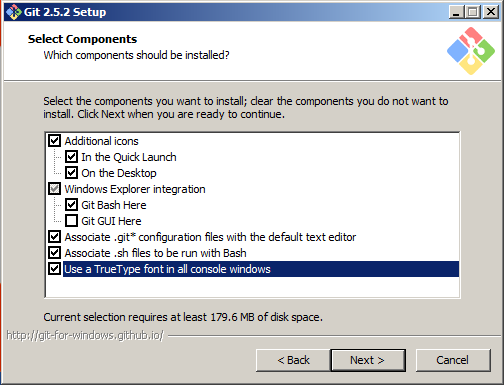
\includegraphics[scale=0.6]{gitwininstall7.png}
\end{center}

\newpage
\item Like in Step 6, just leave the default value.
\begin{center}
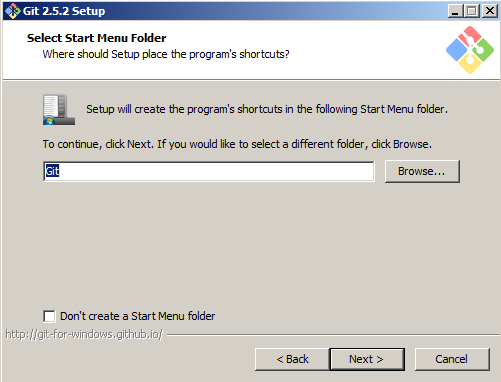
\includegraphics[scale=0.6]{gitwininstall8.png}
\end{center}

\item You can leave this option on the `Use Git from Git Bash only' option, or
    you can be risky and use one of the other two options. It is preferable that
    you only use Git from Git Bash to not alter the rest of the Windows system.
\begin{center}
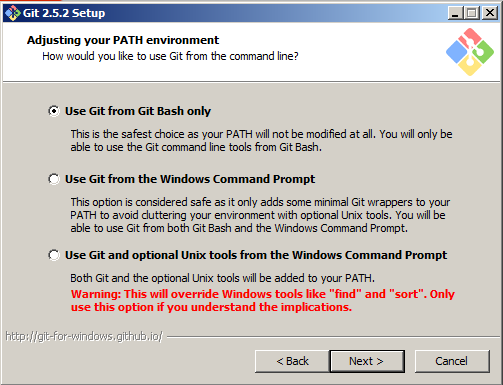
\includegraphics[scale=0.6]{gitwininstall9.png}
\end{center}

\newpage
\item Wait a bit as the loading bar chugs on through\ldots
\begin{center}
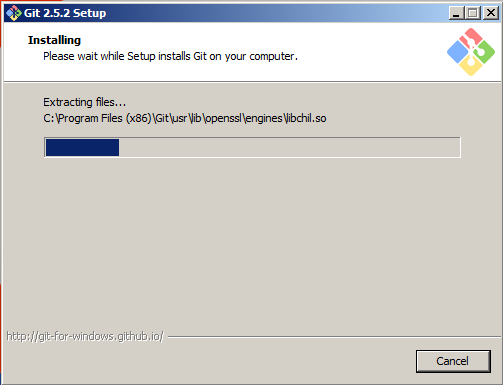
\includegraphics[scale=0.6]{gitwininstall10.png}
\end{center}

\item Uncheck the `View ReleaseNotes.html' checkbox if you want. Release notes
    can be checked here: \url{https://github.com/git-for-windows/git/releases}
\begin{center}
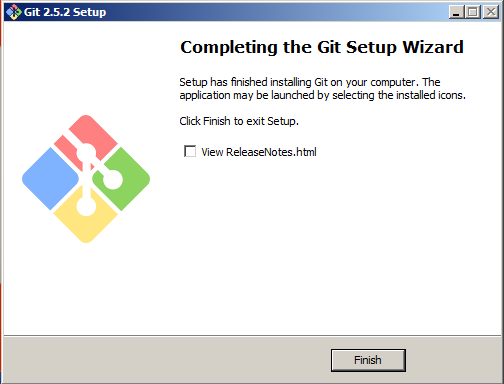
\includegraphics[scale=0.6]{gitwininstall11.png}
\end{center}

\newpage
\item You can open Git Bash through the Desktop shortcut, through the Start
    Menu, or through searching. Just open it.
\begin{center}
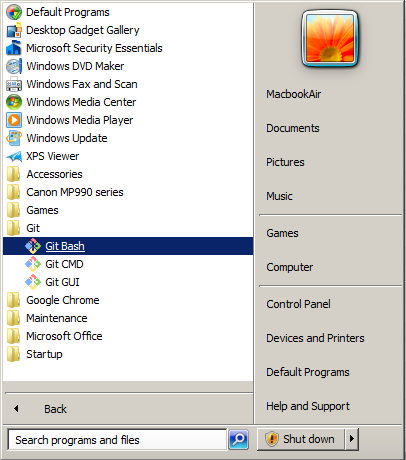
\includegraphics[scale=0.6]{gitwininstall12.png}
\end{center}

\item You should see Git Bash!
\begin{center}
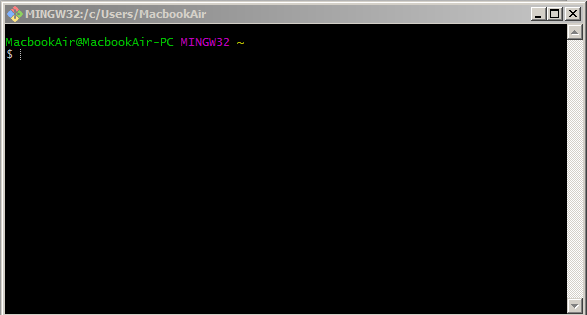
\includegraphics[scale=0.6]{gitwininstall13.png}
\end{center}
\end{enumerate}

\newpage
\subsection{Mac OSX}
There are a number of ways to get \texttt{git} on OSX. If you open Terminal
(Terminal.app), you can type in \texttt{git}, and if it is not currently
installed, it will prompt you to install it. However, XCode does not ship with
the newest version of \texttt{git}, so you can do one of the following:

\subsubsection{Method 1}
Using the GitHub provided installer here: \url{http://git-scm.com/download/mac}

\begin{enumerate}[Step 1.]
\item When you open the installer, you should see this:
\begin{center}
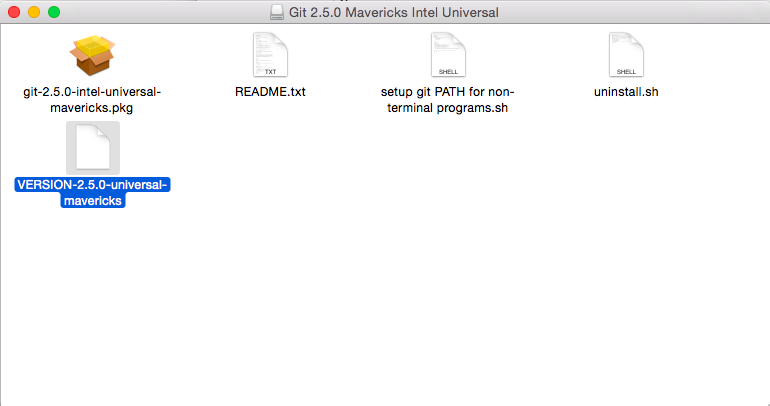
\includegraphics[scale=0.5]{gitmacinstall1.png}
\end{center}
Double click or open the \texttt{.pkg} file (the one that looks like an open box).

\newpage
\item The next step is the default OSX installer introduction. Just hit `Continue.'
\begin{center}
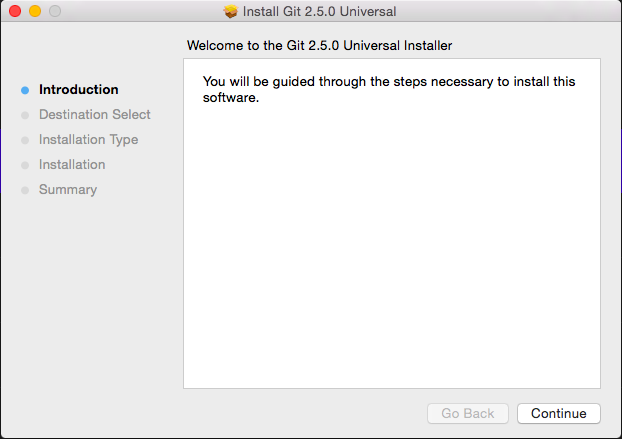
\includegraphics[scale=0.5]{gitmacinstall2.png}
\end{center}

\item You can hit `Customize,' but just hit Install... You're done!
\begin{center}
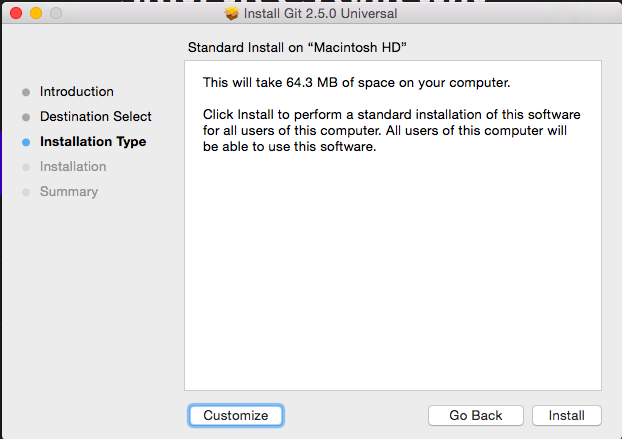
\includegraphics[scale=0.5]{gitmacinstall3.png}
\end{center}
\end{enumerate}

\newpage
\subsubsection{Method 2}
This is the easy, command-line method using a neat command on Mac OSX:
\textit{Homebrew}. Just run the following commands to install Homebrew if you
haven't already installed it:

\begin{center}
\begin{verbatim}
ruby -e "$(curl -fsSL https://raw.githubusercontent.com/Homebrew/install/master/install)"
\end{verbatim}
\end{center}

Then just run the command \verb|brew install git| to install \texttt{git}!

\begin{verbatim}
$ brew install git
==> Downloading https://homebrew.bintray.com/bottles/git-2.5.1.yosemite.bottle.tar.gz
######################################################################## 100.0%
==> Pouring git-2.5.1.yosemite.bottle.tar.gz
==> Caveats
The OS X keychain credential helper has been installed to:
  /usr/local/bin/git-credential-osxkeychain

The "contrib" directory has been installed to:
  /usr/local/share/git-core/contrib

Bash completion has been installed to:
  /usr/local/etc/bash_completion.d

zsh completion has been installed to:
  /usr/local/share/zsh/site-functions
==> Summary
  /usr/local/Cellar/git/2.5.1: 1385 files, 32M
$ git --version
git version 2.3.2 (Apple Git-55)
\end{verbatim}

\subsection{Linux}
Linux is perhaps the OS with the easiest installation process. Just open a
terminal, and using your preferred package manager, install \texttt{git}.
\newline
\verb|$ yum install git|
\newline
\verb|$ sudo apt-get install git|

\section{Local Usage}
\texttt{Git} is a version tracking system for your coding projects. It was made
so that a programmer can easily go through revision history, create multiple
versions of their programs, and move between versions of their programs.

\subsection{Creating a Git Repository}
If you already have a project, you should \texttt{cd} into it. Otherwise, create
a new folder for your project. For this tutorial, I will call my project
\texttt{Git\_Tutorial}. When you are inside your project folder, use the command
\verb|git init|.
\begin{verbatim}
$ mkdir Git_Tutorial
$ cd Git_Tutorial
$ git init
Initialized empty Git repository in Git_Tutorial/.git/
\end{verbatim}

\subsection{Basic Git Commands}
Now that you have a brand new \texttt{git} project. Let's create some files and
add them to the project. (The numbers at the right are for numbering the
commands)
\begin{verbatim}
$ git status                                                          (1)
On branch master
nothing to commit, working directory clean
$ echo "A brand new git project" > README.txt                         (2)
$ ls                                                                  (3)
README.txt
$ git status                                                          (4)
On branch master

Initial commit

Untracked files:
  (use "git add <file>..." to include in what will be committed)

	README.txt

nothing added to commit but untracked files present (use "git add" to track)
$ git add README.txt                                                  (5)
$ git status                                                          (6)
On branch master

Initial commit

Changes to be committed:
  (use "git rm --cached <file>..." to unstage)

	new file:   README.txt

$ git diff --cached                                                   (7)
diff --git a/README.txt b/README.txt
new file mode 100644
index 0000000..c8afd65
--- /dev/null
+++ b/README.txt
@@ -0,0 +1 @@
+A brand new git project
$ git config user.name "elc1798"                                      (8)
$ git config user.email "subliminalmau5@gmail.com"                    (9)
$ git commit -m "My first commit"                                     (10)
$ git status                                                          (11)
On branch master
nothing to commit, working directory clean
$ git log                                                             (12)
commit 58aace97366ac354d164ab5447c32bb42e0ca7bc
Author: elc1798 <subliminalmau5@gmail.com>
Date:   Sat Sep 12 17:35:06 2015 -0400

    My first commit
\end{verbatim}
The above chunk of commands is a lot, so let's break it down.
\begin{enumerate}[\textit{Command }1)]
\item \verb|git status| asks git about the current state of the project. The
    output of this command tells us the current branch of the project we are on
    (master) and the presence of edits to the current version of the project. If
    \verb|git status| says "Nothing to commit, working directory clean" then the
    current state of the project is the same as that of the latest version.
\newpage

\item \verb|echo "A brand new git project" > README.txt| is not a git command.
    \verb|echo| is supposed to print out whatever comes after it to the
    terminal, but the \verb|>| redirects the output into the file
    \verb|README.txt|. The command as a whole creates a new file called
    "README.txt" with the contents "A brand new git project".
\item \verb|ls| is a terminal command to (by default) list out the non-hidden
    contents of the current working directory.
\item We run \verb|git status| again after creating a new file, and our output
    is a bit different! It now shows the commit message of the current version:
    "Initial commit" and lists out the files that are currently not being
    tracked by \verb|git|.a
\item \verb|git add <FILENAME>| will add a file to git's \textit{staging area}.
    The staging area is a list of files with modifications that \verb|git| will
    commit into the new version.
\item Doing \verb|git status| again after we have added "README.txt" to the
    staging area now gives us a "Changes to be committed" section, showing a
    "new file" named "README.txt".
\item \verb|git diff| will show us the differences between non-staged files and
    the state of files of the latest version of the project. \verb|+| represents
    an added line, \verb|-| represents a deleted line. Adding on the
    \verb|--cached| flag (making the command \verb|git diff --cached|) will show
    us the differences between staged files and the state of the files of the
    latest version of the project.
\item \verb|git config [flags] user.name "Your GitHub Username Goes in These Quotes"|
    will change the identity of the default committer of the current
    git project to the specified username. If the flag \verb|--global| is used,
    this will change the name of the default committer of all git projects on
    the local computer.
\item \verb|git config [flags] user.email "Email you registered on GitHub with"|
    will change the default email address used for committing changes of the
    current project to the specified email. If the flag \verb|--global| is used,
    this will change the default email of the default committer of all git
    projects on the local computer.
\item \verb|git commit -m "Commit Message"| will commit staged files and create
    a new version of the project. The \verb|-m| or \verb|--message| flag
    specifies the commit message. A good commit message should explain what was
    changed in the project.
\item Since we just committed, \verb|git status| will tell us that once again
    our working directory is clean.
\item \verb|git log| will show us a list of previous commits, as well as their
    commit messages.
\end{enumerate}

\newpage
\subsection{Keeping Track of and Using Multiple Versions}

\subsubsection{Checking Out}
Git can act like a store. The store contains all the files of your project that
have been committed thus far. We can get a bunch of files from this "store" and
check them out at the cashier! Let's look at an example from our
Github\_Tutorial project:

\begin{verbatim}
$ git status                                           (1)
On branch master
nothing to commit, working directory clean
$ ls                                                   (2)
README.txt
$ cat README.txt                                       (3)
A brand new git project
$ echo "Modify file" > README.txt                      (4)
$ cat README.txt                                       (5)
Modify file
$ git status                                           (6)
On branch master
Changes not staged for commit:
  (use "git add <file>..." to update what will be committed)
  (use "git checkout -- <file>..." to discard changes in working directory)

	modified:   README.txt

no changes added to commit (use "git add" and/or "git commit -a")
$ git checkout README.txt                              (7)
$ git status                                           (8)
On branch master
nothing to commit, working directory clean
$ cat README.txt                                       (9)
A brand new git project
$ echo "Second commit" >> README.txt                   (10) 
$ cat README.txt                                       (11)
A brand new git project
Second commit
$ git add README.txt                                   (12)
$ git commit -m "second commit"                        (13)
[master 57360d8] second commit
 1 file changed, 1 insertion(+)
$ git log --abbrev-commit                              (14)
commit 57360d8
Author: elc1798 <subliminalmau5@gmail.com>
Date:   Sun Sep 20 14:55:37 2015 -0400

    second commit

commit 17e2103
Author: elc1798 <subliminalmau5@gmail.com>
Date:   Sun Sep 20 14:50:15 2015 -0400

    my first commit
$ git checkout 17e2103 README.txt                      (15)
$ cat README.txt                                       (16) 
A brand new git project
$ git checkout HEAD README.txt                         (17)
$ cat README.txt                                       (18)
A brand new git project
Second commit
$ git status                                           (19)
On branch master
nothing to commit, working directory clean
\end{verbatim}

Let's explain this chunk of commands.

\begin{enumerate}[\textit{Command }1)]
\item Like always, we check the local status of our repository with \verb|git status|.
    The output tells us there's nothing modified from the most recent
    commit.

\item Just for demonstration purposes, \verb|ls| tells us the only non-hidden
    file is \verb|README.txt|

\item We display the contents of \verb|README.txt|, which says ``A brand new git
    project'' (from the previous section).

\item We change the contents of \verb|README.txt| to ``Modify file''

\item Verify the contents changed with \verb|cat|

\item \verb|git status| tells us that \verb|README.txt| is modified.

\item \verb|git checkout README.txt| is our `checking out.' \verb|git checkout <FILENAME>|
    will take a file called \verb|<FILENAME>| from the most recent
    version of the project and put that into the current working directory.

\item \verb|git status| tells us that the local modifications have been
    overwritten and the working directory is clean.

\item Verify the contents changed with \verb|cat|

\item We changed the contents of \verb|README.txt| by adding the second line
    ``Second commit.''

\item Verify the contents changed with \verb|cat|

\item We add the modified file to the trackers with \verb|git add|.

\item We commit the change with the message ``second commit.''

\item \verb|git log --abbrev-commit| shows us a list of previous commits, with
    each commit abbreviated.

\item We once again `check out' \verb|README.txt| with \verb|git checkout|,
    except this time we specify the commit, so now the local working directory's
    version of \verb|README.txt| is the same as that in commit \verb|17e2103|.
    By doing \verb|git checkout <COMMIT> <FILENAME>|, the local file called
    \verb|FILENAME| will be reverted to its version in \verb|COMMIT|

\item Verify the contents changed with \verb|cat|

\item We can also revert to the latest commit by using \verb|git checkout HEAD README.txt|,
    we change the file to the most current commit.

\item Verify the contents changed with \verb|cat|

\item We can now see that the working directory is up to date with \verb|git status|.
\end{enumerate}

\subsubsection{Branches}
A Git project is like a tree. There is a main trunk with the current public
release, and there are different branches with other versions of the project. To
see the options available for the \verb|branch| feature of \verb|git|, use the
command: \texttt{git branch -h}\\
You can use the command \verb|git branch -a| to list all the branches of a git
project.

\begin{verbatim}
\end{verbatim}

As usual, let's break down the chunk of commands above.

\end{document}
